\documentclass[11pt,a4paper]{article}
\usepackage[margin=24mm,headheight=15pt]{geometry}
\usepackage{amsmath,amssymb,amsthm,fontspec,unicode-math}
\setmainfont{texgyrepagella-regular.otf}[BoldFont=texgyrepagella-bold.otf,ItalicFont=texgyrepagella-italic.otf,BoldItalicFont=texgyrepagella-bolditalic.otf]
\setmathfont{texgyrepagella-math.otf}
\setmonofont{lmmono10-regular.otf}
\usepackage{booktabs,array,tabularx,xcolor,graphicx,fancyhdr,xurl,tikz}
\usetikzlibrary{arrows.meta,calc}
\definecolor{ink}{RGB}{25,54,76}
\definecolor{teal}{RGB}{0,113,116}
\definecolor{rust}{RGB}{164,73,38}
\usepackage[colorlinks=true,linkcolor=ink,citecolor=ink,urlcolor=ink]{hyperref}
\hypersetup{pdftitle={Dipole Fields and Passive Loop Readout in the Tri-Octagon Model},pdfauthor={Hilmir Frímann Halldórsson},pdfsubject={GM04--GM06; research edition v0.1; author-approved repository research edition; project-internal GPT review}}
\pagestyle{fancy}\fancyhf{}
\fancyhead[L]{\small Tri-Octagon: dipole fields and loop readout}
\fancyhead[R]{\small Research edition v0.1}
\fancyfoot[C]{\thepage}
\setlength{\parindent}{0pt}\setlength{\parskip}{4pt}
\setlength{\emergencystretch}{3em}\raggedbottom
\clubpenalty=10000\widowpenalty=10000\displaywidowpenalty=10000
\numberwithin{equation}{section}
\newtheorem{theorem}{Theorem}[section]
\newtheorem{proposition}[theorem]{Proposition}
\newtheorem{corollary}[theorem]{Corollary}
\theoremstyle{remark}\newtheorem{remark}[theorem]{Remark}
\newcommand{\R}{\mathbb R}\newcommand{\C}{\mathbb C}
\newcommand{\dd}{\,\mathrm d}\newcommand{\ii}{\mathrm i}
\newcommand{\ex}{e_x}\newcommand{\ey}{e_y}\newcommand{\ez}{e_z}
\newcommand{\norm}[1]{\left\lVert#1\right\rVert}
\newcommand{\abs}[1]{\left|#1\right|}
\newcommand{\diag}{\operatorname{diag}}
\newcommand{\Hess}{\operatorname{Hess}}
\newcommand{\Argz}{\operatorname{Arg}_0}
\newcolumntype{Y}{>{\raggedright\arraybackslash}X}
\begin{document}
\begin{titlepage}
{\small\color{ink} TRI-OCTAGON MATHEMATICAL RESEARCH\par}
\vspace{10mm}
{\LARGE\bfseries\raggedright Dipole Fields and Passive Loop Readout\\[2mm]
in the Tri-Octagon Model\par}
\vspace{8mm}
{\large Hilmir Frímann Halldórsson\par}
\vspace{3mm}
{Research edition v0.1 \quad 20 November 2026\par}
{\small Author-approved repository research edition.\par}
\vspace{8mm}
\begin{abstract}
A steady tangent-encoded circulation on an adopted Tri-Octagon carrier circle produces a vector observation whose spatial curl has the dipole angular tensor and inverse-cube leading decay. We develop two signed tests from that exterior kernel. In the coaxial test the vector observation vanishes at the receiving circle's center, yet its oriented rim integral has the source sign at every positive pair of radii and nonzero axial separation. Rotational symmetry makes one ideal tangential rim sample sufficient in this special case.

The native map does not itself assign the required carrier means. A proposed three-loop source impulse lifts the native planar observable \(W\) to unique minimum-storage means under equal weights. Its exact Fourier launch costs \(6.768750025\times10^{-9}L\alpha^2\); conjugation reverses the means at the same cost. A finite receiving circle on a registered rigid copy distinguishes the two launches for every \(R\ge100w\), with a relative error certificate below one third. At \(R=100w\), 1,024 additional exact contour samples also suffice. The circle center, body-center probe, finite-area component, source offsets and complete delay window remain distinct. The source impulse and contour readout are explicit additions. An internal source donor and a law changing a second native triad remain open.
\end{abstract}
\vfill
{\small\textbf{Status and provenance.} This manuscript assembles the project-internally accepted GM04, corrected GM05 and reviewed GM06 investigations. It incorporates the common-offset and latest-delay corrections. After GPT review and the two wording corrections, the author approved repository publication. The tests are mathematical consequences of specified equations; no external peer review or physical validation is claimed. GPT supplied proposals and review; Codex supplied source verification, mathematical checks and manuscript preparation under the author's direction.}
\end{titlepage}
\setcounter{page}{2}
\section{A silent center and a signed rim}\label{sec:coaxial}
The simplest test separates a point observation from a measurement around a loop. A steady source circle and a coaxial receiving circle can have a zero vector observation at the receiving circle's center while the oriented rim integral is strictly signed. This is the first result to explain. We then ask how a native state can prepare the source and whether the signed signal survives at a receiver with the model's actual finite radius.

The preceding GM01--GM03 paper imposed Newtonian and magnetostatic field laws through an explicit source dictionary and studied interaction-driven feedback~\cite{GM123}. The present paper follows a different chain: the adopted C6 exterior kernel, a prepared carrier, a proposed native-to-mean impulse, and a passive contour readout~\cite{GM04,GM05,GM06}. A line circle has finite-radius corrections; it is not the radial magnetization profile for which the earlier paper obtained an exact external dipole interaction.

\subsection{The adopted observation and its orientation}
Write a source circle and its oriented unit tangent as
\begin{equation}\label{eq:sourcecircle}
\gamma(\phi)=Y+a(\cos\phi\,e_1+\sin\phi\,e_2),\quad
\widehat t(\phi)=-\sin\phi\,e_1+\cos\phi\,e_2,\quad
\nu=e_1\times e_2,
\end{equation}
where \(e_1,e_2\) are orthonormal, \(a>0\), and \(L=2\pi a\).
C6 adopts a straight delay, tangent encoding and inverse-distance kernel~\cite{PAIRII,INT}:
\begin{align}
U(P,t)&=\frac{g_o}{4\pi}\int_0^L
\frac{p(s,t-d_P(s)/c_e)}{d_P(s)}\dd s,\notag\\
V(P,t)&=\frac{g_o}{4\pi}\int_0^L
\frac{r_c(s,t-d_P(s)/c_e)\widehat t(s)}{d_P(s)}\dd s,
\quad d_P(s)=|P-\gamma(s)|. \label{eq:C6}
\end{align}
Here \(g_o,c_e>0\). A registered point probe returns \((U,B^TV)\) for a known orthonormal frame B. The tangent-encoded \(r_c\widehat t\) is not assigned material electric current, and C6 is a passive observation without loading.

Prepare the steady source \(p=0,r_c=j\), with the corresponding constant history. Then
\begin{equation}\label{eq:staticV}
V(P)=\frac{g_oj}{4\pi}\oint_{\Gamma}\frac{\dd\gamma}{|P-\gamma|},
\qquad H(P):=\nabla_P\times V(P).
\end{equation}
The symbol H denotes this mathematical curl. Identifying it with a measured magnetic field would require calibration beyond the adopted kernel.

\begin{figure}[tbp]
\centering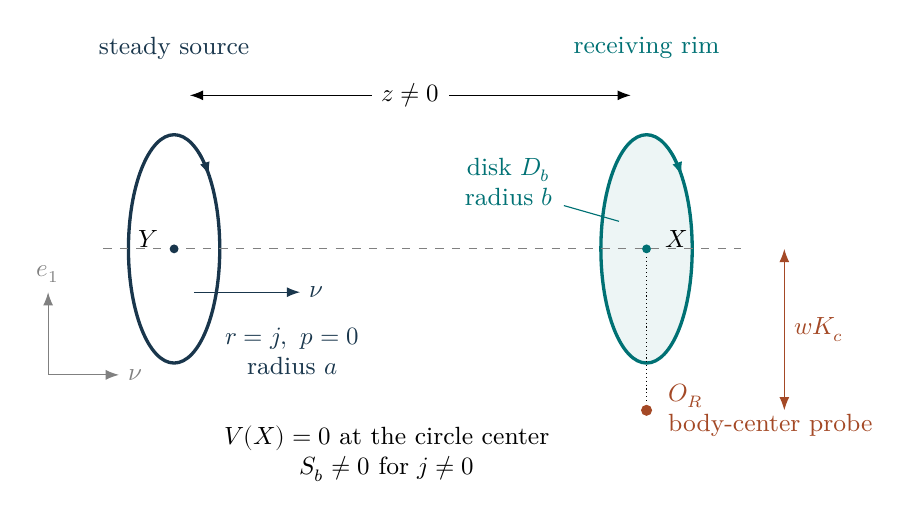
\begin{tikzpicture}[x=1cm,y=1cm,>=Latex,font=\small]
\fill[teal!7] (6,0) ellipse (.58 and 1.45);
\draw[ink,very thick] (0,0) ellipse (.58 and 1.45);
\draw[teal,very thick] (6,0) ellipse (.58 and 1.45);
\draw[dashed,gray] (-.9,0)--(7.2,0);
\draw[->,ink] (0,1.45) arc[start angle=90,end angle=40,x radius=.58,y radius=1.45];
\draw[->,teal] (6,1.45) arc[start angle=90,end angle=40,x radius=.58,y radius=1.45];
\draw[<->] (.2,1.95)--node[fill=white] {$z\ne0$}(5.8,1.95);
\fill[ink] (0,0) circle(1.6pt);
\fill[teal] (6,0) circle(1.6pt);
\node[anchor=east] at(-.15,.12) {$Y$};
\node[anchor=west] at(6.12,.12) {$X$};
\node[ink] at(0,2.55) {steady source};
\node[teal] at(6,2.55) {receiving rim};
\draw[->,ink] (.25,-.55)--(1.6,-.55) node[right] {$\nu$};
\node[ink,align=center] at(1.5,-1.3) {$r=j,\ p=0$\\radius $a$};
\node[teal,align=center] at(4.25,.85) {disk $D_b$\\radius $b$};
\draw[teal] (4.95,.55)--(5.65,.35);
\fill[rust] (6,-2.05) circle(2pt);
\draw[densely dotted] (6,-.1)--(6,-1.95);
\node[anchor=west,rust,align=left] at(6.15,-2.05) {$O_R$\\body-center probe};
\draw[<->,rust] (7.75,0)--node[right] {$wK_c$}(7.75,-2.05);
\draw[->,gray] (-1.6,-1.6)--(-1.6,-.55) node[above] {$e_1$};
\draw[->,gray] (-1.6,-1.6)--(-.7,-1.6) node[right] {$\nu$};
\node[align=center] at(2.7,-2.6) {$V(X)=0$ at the circle center\\$S_b\ne0$ for $j\ne0$};
\end{tikzpicture}

\caption{Coaxial test, shown schematically in an oblique projection; not to scale. Increasing source and receiver angles use the same oriented plane, with \(\nu=e_1\times e_2\) pointing along the common axis. The receiving disk center X is on that axis. Its body-center probe \(O_R=X-wK_ce_1\) is displaced and can already read a nonzero V. The disk is an integration device, not a material panel.}\label{fig:coaxial}
\end{figure}

\subsection{The finite receiving circle}
Place the receiving contour at
\begin{equation}\label{eq:coaxreceiver}
X=Y+z\nu,\qquad q(\theta)=X+b(\cos\theta\,e_1+\sin\theta\,e_2),
\quad t(\theta)=-\sin\theta\,e_1+\cos\theta\,e_2,
\end{equation}
with \(b>0,z\ne0\). Increasing theta fixes the measured orientation. Its area-normalized signed reading is
\begin{equation}\label{eq:sensor}
S_b(X,\nu)=\frac1{\pi b^2}\oint_{\partial D_b}V\cdot\dd\ell
=\frac1{\pi b}\int_0^{2\pi}V(q(\theta))\cdot t(\theta)\dd\theta.
\end{equation}
At X every source point has distance \(\sqrt{a^2+z^2}\), and \(\oint\dd\gamma=0\); consequently \(U(X)=V(X)=0\), for both an empty source and every constant j.

\begin{theorem}[Finite coaxial sign]\label{thm:coaxial}
With the orientation above, \(S_b\) has the sign of j for every \(a,b>0,z\ne0\). It vanishes at \(j=0\). Reversing j or the receiving traversal reverses the reading.
\end{theorem}
\begin{proof}
The double line integral has tangent pairing \(ab\cos(\phi-\theta)\) and squared distance
\(a^2+b^2+z^2-2ab\cos(\phi-\theta)\). Rotational symmetry removes the theta integral, giving
\begin{equation}\label{eq:coaxexact}
S_b=\frac{g_oj a}{2\pi b}\int_0^{2\pi}
\frac{\cos\phi}{\sqrt{C-q_0\cos\phi}}\dd\phi,\qquad
C=a^2+b^2+z^2,\quad q_0=2ab.
\end{equation}
Since \(C-q_0=(a-b)^2+z^2>0\), pairing opposite cosines rewrites the integral as
\begin{equation}\label{eq:positivepair}
\int_{-\pi/2}^{\pi/2}\cos\phi
\left[(C-q_0\cos\phi)^{-1/2}-(C+q_0\cos\phi)^{-1/2}\right]\dd\phi>0.
\end{equation}
The integrand is positive in the interval interior. Linearity in j and orientation of the line integral prove the remaining statements.
\end{proof}

\begin{corollary}[One rim sample in this control]\label{cor:onesample}
For this steady aligned coaxial source only, every rim point gives
\begin{equation}\label{eq:onesample}
S_b=\frac2b\,V(q(\theta))\cdot t(\theta).
\end{equation}
\end{corollary}
\begin{proof}
Rotation about the common axis carries both \(V(q(\theta))\) and \(t(\theta)\) by the same rotation. Their dot product is constant; substitute it into \eqref{eq:sensor}.
\end{proof}
One ideal signed tangential sample thus suffices in this symmetric control. This is not a universal replacement for a contour or the later three-source sampling certificate.

Integrating the derivative of \(x^{-1/2}\) in the paired expression gives, for \(j>0\),
\begin{equation}\label{eq:coaxbounds}
\frac{g_oj a^2}{2[z^2+(a+b)^2]^{3/2}}
\le S_b\le
\frac{g_oj a^2}{2[z^2+(a-b)^2]^{3/2}}.
\end{equation}
The positivity is exact at finite radii. The bounds are conservative.

\subsection{A circle on an actual copy}
The established geometry supplies~\cite{PAIR}
\begin{equation}\label{eq:geometryconstants}
K_c=\frac{\sqrt3}{12}+\frac{\sqrt6}{4},\qquad
R_\Gamma=\frac{\sqrt7K_c}{2(1+\sqrt3/2)},\qquad
a=b=wR_\Gamma,\quad R_\Gamma=0.53645209718\ldots,
\end{equation}
where w is common host width. In the published orientation, \(Y=O+wK_c\ey\), \(e_1=\ey,e_2=\ez,\nu=\ex\). Translate an unrotated same-width copy by \(z\ex\). Its circle center is \(X=Y+z\ex\), but its body center is \(O_R=O+z\ex=X-wK_c\ey\).

This is an explicit rigid test placement, preserving the established circle and full-copy geometry; it is not one of the published H/R array fixtures. The zero reading is at the \emph{circle center}, not generally at the existing body-center probe. At the benchmark \(z=4w\), enclosing balls of radius \(w(K_c+R_\Gamma)<2w\) separate the two full copies and all their circles. The all-\(z\ne0\) integral theorem alone does not assert full-body noncollision at small z.

\section{The curl and its dipole tensor}\label{sec:field}
On every compact region separated from the source wire, differentiation under \eqref{eq:staticV} gives
\begin{equation}\label{eq:curl}
H(P)=\frac{g_oj}{4\pi}\oint_\Gamma
\frac{\dd\gamma\times(P-\gamma)}{|P-\gamma|^3}.
\end{equation}
The sign follows from \(\nabla_P|P-\gamma|^{-1}=-(P-\gamma)/|P-\gamma|^3\). On the axis,
\begin{equation}\label{eq:axis}
V(Y+z\nu)=0,\qquad
H(Y+z\nu)=\frac{g_oj a^2}{2(a^2+z^2)^{3/2}}\nu.
\end{equation}
Taking a curl after restricting V to its zero axial values would incorrectly discard the transverse derivatives. The spatial derivative must be taken first.

For a general point \(P=Y+rn\), \(n\in S^2\), define
\(m_\Gamma=\pi a^2j\nu\). The exact accepted field estimate is~\cite[sections 2--3]{GM04}
\begin{equation}\label{eq:dipole}
H(Y+rn)=\frac{g_o}{4\pi r^3}\{3n(n\cdot m_\Gamma)-m_\Gamma\}
+\mathcal R(r,n),
\end{equation}
\begin{equation}\label{eq:remainder}
\norm{\mathcal R(r,n)}\le
\frac{3g_o|j|a^4}{2(r-a)^5}\quad(r>a),\qquad
\norm{\mathcal R(r,n)}\le\frac{48g_o|j|a^4}{r^5}\quad(r\ge2a).
\end{equation}
These are uniform absolute bounds, not relative smallness claims at \(r=2a\).

To see the tensor and the order without differentiating an uncontrolled asymptotic series, use the filled source disk only as an integration device. For \(R=P-Y\), set
\(\Phi(R)=\int_{D_a}|R-\rho|^{-1}\dd A_\rho\). Stokes' theorem componentwise gives, outside that disk,
\begin{equation}\label{eq:diskH}
V=\frac{g_oj}{4\pi}\nabla\Phi\times\nu,\qquad
H=\frac{g_oj}{4\pi}\int_{D_a}\Hess(|R-\rho|^{-1})\nu\dd A_\rho.
\end{equation}
The center Hessian is
\begin{equation}\label{eq:kernelG}
G(R)=\Hess(|R|^{-1})=\frac{3nn^T-I}{r^3}.
\end{equation}
The disk's first moment vanishes. The bound
\(\norm{D_v^2G(x)}_{\rm op}\le24|v|^2/|x|^5\), proved in Appendix~\ref{app:kernel}, and
\(\int_{D_a}|\rho|^2\dd A=\pi a^4/2\) yield \eqref{eq:remainder} by Taylor's integral remainder. Centered symmetry removes the \(r^{-4}\) term.

The leading angular factors are \(2m_\Gamma\) along either axial direction and \(-m_\Gamma\) in the equatorial plane, with general tensor \(3nn^T-I\). This is the magnetic-dipole pattern of the curl of the adopted vector observation. In inherited units,
\([V]=\mathrm U,\ [H]=\mathrm U/\mathrm L,\ [m_\Gamma]=\mathrm U\mathrm L^2\).
Neither the SI coupling nor a receiver law follows from that pattern.

\subsection{Finite-area measurement and clearance}\label{sec:area}
If V is \(C^1\) on a neighborhood of the entire receiving disk, the proposed readout obeys
\begin{equation}\label{eq:stokes}
S_b(X,u)=\frac1{\pi b^2}\int_{D_b}H(P)\cdot u\dd A.
\end{equation}
For stationary line sources, positive clearance of the \emph{whole disk} from every source wire ensures smoothness. Boundary clearance alone is insufficient when a wire pierces the interior. The disk is not an assumed physical surface.

If \(M_2=\sup_{D_b}\norm{\nabla^2(H\cdot u)}_{\rm op}\), centered Taylor averaging gives
\begin{equation}\label{eq:areaerror}
|S_b-H(X)\cdot u|\le\frac{b^2M_2}{4}.
\end{equation}
The linear term averages to zero and the average of \(|P-X|^2\) is \(b^2/2\). For equal source radii a, write \(J_*=\sum_i|j_i|\). If the receiving disk is separated from the filled source disks by \(\delta_D>0\), \eqref{eq:diskH} and the same Hessian derivative bound imply
\begin{equation}\label{eq:diskaveragebound}
M_2\le\frac{6g_oa^2J_*}{\delta_D^5},\qquad
|S_b-H(X)\cdot u|\le\frac{3g_oa^2b^2J_*}{2\delta_D^5}.
\end{equation}
The stronger filled-disk separation is a sufficient condition for this estimate. In the coaxial test it is at least \(|z|\). Table~\ref{tab:coax} keeps the actual finite radius rather than substituting a point receiver.

\begin{table}[tbp]\centering\small
\begin{tabular}{@{}rrrr@{}}\toprule
\(z/w\)&\(S_b\)&\(H(X)\cdot\nu\)&Bound on their difference\\\midrule
2&0.0148118125093&0.0162062684439&0.00388208527065\\
4&0.00213341379003&0.00218896603617&0.000121315164708\\
8&0.000277297390899&0.000279151038132&0.00000379109889712\\\bottomrule
\end{tabular}
\caption{Saved GM06 quadrature at \(w=g_o=j=1\) and \(a=b=R_\Gamma\). The bound is \(3g_o|j|a^2b^2/(2|z|^5)\). Single angular integration, double line integration and disk integration agree in the preserved evidence. These values corroborate the analytic sign proof; they do not establish it.}\label{tab:coax}
\end{table}

\section{From a native moment to three carrier means}\label{sec:source}
The preceding field calculation starts from a steady circulation. It does not show that native evolution generates that circulation. This section states the two inherited obstructions and the particular source impulse assessed in GM05.

\subsection{Native observables and the old carrier interface}
Paper G defines the channel-space area C and its ambient axial attachment W~\cite{G}:
\begin{equation}\label{eq:TC}
C=\Re\Omega\times\Im\Omega,\qquad W=TC,\qquad
T=\begin{pmatrix}-1/2&1&-1/2\\-\sqrt3/2&0&\sqrt3/2\\0&0&0\end{pmatrix}.
\end{equation}
W is planar; it is different from the host width w. In the geometric source order,
\begin{equation}\label{eq:threegeometry}
u_k=R_z(2\pi k/3)\ey,\quad
Y_k=O+wK_cu_k,\quad
\nu_k=u_k\times\ez,\quad T=[\nu_2\ \nu_0\ \nu_1].
\end{equation}
The source weights A, B, C therefore correspond to circles 2, 0, 1. Geometry supplies three possible circles with distinct centers; the retained C1/RX dynamics instantiates only circle 0.

For the periodic adopted carrier~\cite{INT,RX},
\begin{equation}\label{eq:C1}
p_t+c(r_c)_s=g_c,\qquad (r_c)_t+cp_s=0,\qquad
j=L^{-1}\int_0^Lr_c\dd s.
\end{equation}
Periodic integration gives \(\dot j=0\). RX's native-first jump changes the native state only, leaving the carrier and old receiver unchanged. The mean is therefore invariant across inherited jumps as well. For every instantaneous profile on a circle,
\begin{equation}\label{eq:meanmoment}
\frac12\int(\gamma-Y)\times(r_c\widehat t)\dd s=\pi a^2j\nu.
\end{equation}
Thus an initially empty retained circle cannot gain this centered moment under C1/RX. This does not imply that its whole state or exterior observation remains zero. The mean statement extends to periodic L2 mild solutions by the bounded mean functional.

There is also an information obstruction. With positive fixed gains, the old source uses
\begin{equation}\label{eq:ports}
f=KC,\qquad
K=\kappa_{\rm in}\lambda_g
\begin{pmatrix}n_+^T\\n_-^T\end{pmatrix}R_z(\delta_g),
\qquad n_\pm=(2\ey\pm\sqrt3\ez)/\sqrt7.
\end{equation}
In channel coordinates take \(v=(\cos\delta_g,-\sin\delta_g,0)^T\).
Then
\begin{equation}\label{eq:portnull}
Kv=0,\qquad |Tv|^2=1+\tfrac12\sin(2\delta_g)\ge\tfrac12.
\end{equation}
The exact states \(\Omega_\pm=E_3\pm\ii(v\times E_3)\), where \(E_3\) is the third channel basis vector, have intensity 2, \(C_\pm=\pm v\), equal zero old ports and opposite nonzero W. No instantaneous function of those two ports determines W. These two states are not asserted to be adjacent native iterates or to retain equal ports after arbitrary later native jumps.

WT changes the mean equation through its actual returning waves~\cite{WT,GM04}. If \(b_r\) is the incoming backward component and M is total receiving-arc length, its equation is
\begin{equation}\label{eq:WTmean}
L\dot j=-\kappa^2Lj+
\frac{\sqrt2\kappa}{\sqrt M}\int_{S_L\times G}b_r(s,X,t)\dd s\dd\ell_X.
\end{equation}
This is history-dependent feedback, not a universal assignment from W. Entirely empty carrier, transport and receiver preparation has no return before \(2\theta_-\), so its initially zero mean stays zero in that startup interval. WT native jumps still leave carrier/transport stocks unchanged. A single fixed-normal circle also cannot represent W directions outside its normal line.

\subsection{The explicitly added source impulse}
GM05 instantiates three equal-radius carrier states and reads W directly. Define
\begin{equation}\label{eq:lift}
e=(1,1,1)^T,\quad P=I-ee^T/3,\quad
D=\tfrac23T^T,\quad TD=\diag(1,1,0),\quad DT=P.
\end{equation}
For real symbolic \(\alpha\), the target is \(Tj=\alpha W\). Its full family is
\begin{equation}\label{eq:family}
j=\alpha DW+\beta e,\qquad
\frac L2|j|^2=\frac{L\alpha^2}{3}|W|^2+\frac{3L}{2}\beta^2.
\end{equation}
Indeed \(TDW=W\) on Paper G's plane and \(\ker T=\R e\); the two components of j are orthogonal. Equal positive lengths and storage weights select the unique minimum at \(\beta=0\):
\begin{equation}\label{eq:jstar}
j_*=\alpha DW=\frac{\alpha}{3}
(-W_x-\sqrt3W_y,\ 2W_x,\ -W_x+\sqrt3W_y)^T.
\end{equation}
The scale has units of loop mean per unit W and is not RX's native-storage scale \(\alpha_N\). Its sign fixes alignment or reversal. Unequal weights would change the minimization problem.

At an ordinary native update the hypothesis adds
\begin{equation}\label{eq:jump}
\Delta j=\alpha D(W^+-W^-),\qquad
r_i^+(s)=r_i^-(s)+\Delta j_i,\qquad p_i^+=p_i^- .
\end{equation}
This is a prescribed uniform, simultaneous actuation, not a consequence of the old p-source ports. It uses information those ports lose. Writing \(r_i=j_i+\widetilde r_i\), with \(\int\widetilde r_i=0\), shows that every zero-mean profile is preserved at the jump.

\begin{proposition}[Tracking is conditional]\label{prop:tracking}
The mismatch \(q=j-\alpha DW\), the visible mismatch \(Tj-\alpha W\), and the common mean \(e^Tj/3\) are unchanged by \eqref{eq:jump}. Correct minimum initialization tracks across the jump. Existing mismatch is not repaired.
\end{proposition}
\begin{proof}
Subtract \(\alpha DW^+\) from \(j^-+\alpha D(W^+-W^-)\). The result is \(j^--\alpha DW^-\). Also \(e^TD=0\).
\end{proof}
The increment is the minimum-norm increment with its required visible change, not an unconditional reset to minimum endpoint storage. Empty carriers are matched only when \(\alpha W^-=0\).

Between jumps, active exchange can change W while preserving j. For an exact RX witness at unit source gains and yaw zero, take \(a_N=E_3,b_N=E_1\), old port output \(y=(1,1)^T\), and \(\mu=\eta_N/(2\alpha_N)>0\). Its actual native exchange equation gives
\begin{equation}\label{eq:interjump}
K^Ty=4E_2/\sqrt7,\quad
\dot a_N=-4\mu E_3/\sqrt7,\quad
\dot b_N=-4\mu E_1/\sqrt7,\quad
W=\ex,\quad \dot W=-8\mu\ex/\sqrt7.
\end{equation}
The stated y is attained by \(p=(b_++b_-)/\|b_+\|_2^2\) for the retained disjoint equal tents. A later jump preserves the resulting error. Full plateau tracking is therefore a source-off, native-held comparison, not a consequence of arbitrary loaded evolution.

\subsection{Exact Fourier launch and its cost}
Retain the ordinary native map, with simultaneous stages~\cite{RX}:
\begin{align}
\widetilde\Omega_i&=\Omega_i+\epsilon(k_i-|\Omega_i|^2)\Omega_i
+g\sum_{j\ne i}(\Omega_j-\Omega_i),\notag\\
F_i(\Omega)&=e^{\ii\delta_i}\widetilde\Omega_i,\qquad
\delta_i=\lambda\sum_{j\ne i}\sin\{3(\Argz\widetilde\Omega_j-\Argz\widetilde\Omega_i)\}.
\label{eq:F}
\end{align}
Here \(\Argz(0)=0\), and exact zero components stay zero. At
\begin{equation}\label{eq:tuple}
\epsilon=\tfrac1{10},\quad g=\tfrac1{60},\quad\lambda=\tfrac1{300},
\quad k=(999/1000,1,1001/1000),
\end{equation}
take \(\Omega^-=(1,\omega,\omega^2)\), \(\omega=e^{-2\pi\ii/3}\).
All prestage multipliers are positive and all triple-angle phase kicks vanish:
\begin{equation}\label{eq:Fourier}
\Omega_i^+=\frac{(9499,9500,9501)_i}{10000}\Omega_i^-,
\quad W^-=0,\quad
W^+=W_0=\left(\frac{\sqrt3}{200000000},\frac{57}{400000},0\right)^T.
\end{equation}
Thus the empty matched carriers launch to
\begin{equation}\label{eq:launch}
\boxed{j^+=\frac{\alpha\sqrt3}{600000000}(-28501,2,28499)^T,\qquad
m_{\rm tot}=\pi a^2Tj^+=\pi a^2\alpha W_0.}
\end{equation}
For positive alpha the circle-2 mean is negative and the circle-0 and circle-1 means are positive. These are orientation signs, not negative energies. Conjugating the native preparation conjugates its update and reverses every mean.

For arbitrary square-integrable preprofiles, the exact inherited carrier-storage change is
\begin{equation}\label{eq:work}
\boxed{\Delta E_C=L\left(j^-\cdot\Delta j+\tfrac12|\Delta j|^2\right).}
\end{equation}
Expand the square of \(r_i^-+\Delta j_i\), integrate, and use the definition of the means; p and all zero-mean profiles contribute zero jump change. For matched minimum endpoints,
\begin{equation}\label{eq:matchedwork}
E_{\rm means}=\frac{L\alpha^2}{3}|W|^2,\qquad
\Delta E_C=\frac{L\alpha^2}{3}(|W^+|^2-|W^-|^2).
\end{equation}
The empty Fourier launch has the strictly positive cost, for \(\alpha\ne0\),
\begin{equation}\label{eq:launchcost}
\boxed{\Delta E_C=
\frac{270750001}{40000000000000000}L\alpha^2
=6.768750025\times10^{-9}L\alpha^2.}
\end{equation}
The conjugate costs exactly the same. General signed work can be negative, in which case the actuation receives carrier energy.

\subsection{Common offsets and the unassigned payer}
The reviewed offset correction is essential~\cite[section 4, corrected]{GM05}. If
\(j^-=\alpha DW^-+\beta_0e\), reversing W yields
\begin{equation}\label{eq:offsetreversal}
j^+=-j^-+2\beta_0e,\qquad \Delta E_C=0.
\end{equation}
Only the W-driven part reverses. Taking W to zero leaves \(3L\beta_0^2/2\) stored. Separately adding \(\beta e\) changes storage by
\begin{equation}\label{eq:offsetwork}
\Delta E_{\rm offset}=3L\beta_0\beta+\tfrac32L\beta^2.
\end{equation}
For arbitrary mismatch q the work has the additional term
\(L\alpha q\cdot D(W^+-W^-)\) relative to \eqref{eq:matchedwork}.

The common mode also matters physically within the comparison: it leaves \(Tj\) unchanged but changes the finite-distance field of separated loops. The raw alternative \(j=\alpha C\) differs from the minimum by \(\alpha(e^TC)e/3\). At the Fourier entrance \(C=-(\sqrt3/2)e\), W is zero: the minimum is empty, whereas the raw assignment stores \(9L\alpha^2/8\). Matching the aggregate dipole does not match the whole field.

No inherited equation supplies the extra work in \eqref{eq:work}. The old hybrid changes only native trial storage by \(\alpha_N\Delta I/2\); appending the impulse gives \(\Delta H_{\rm tot}=\alpha_N\Delta I/2+\Delta E_C\), without an automatic cancellation. At the same tuple, the real aligned entrance \(\Omega=(1,1,1)\) has \(F\Omega=(9999/10000,1,10001/10000)\), zero W at both endpoints and \(\Delta I=1/50000000>0\). Its loop work is zero. The native account is not a universal donor identity. GM01--GM03 stores balance their specified pair interaction, not this newly added loop energy. A balancing ledger entry would not identify a material donor, finite reserve or feedback law.

\section{The native launch at a registered finite receiver}\label{sec:receiver}
Hold the three source profiles in \eqref{eq:launch} at their constant source-off endpoints, with p zero. The following result concerns that prepared plateau. Active later RX or WT evolution would require its actual histories and is not silently frozen by the mathematics.

\subsection{Placement and the measured component}
Choose a same-width receiving copy with the already defined proper frame
\begin{equation}\label{eq:receiverplacement}
Q=B(\pi/2)=[\ey,\ez,\ex],\qquad
O_R=O+(R-wK_c)\ez.
\end{equation}
Its local circle 0 has
\begin{equation}\label{eq:nativecontour}
X=O_R+wK_cQ\ey=O+R\ez,\qquad
q(\theta)=X+b(\cos\theta\,\ez+\sin\theta\,\ex),\quad
b=a=wR_\Gamma,\quad u=\ey.
\end{equation}
This rigid test placement uses a published orientation but not a published positive-radius H/R ring position. It changes neither the shell shape nor the loop radius. Circle-center X and body-center \(O_R\) differ, as Figure~\ref{fig:native} shows.

\begin{figure}[tbp]
\centering\resizebox{0.90\textwidth}{!}{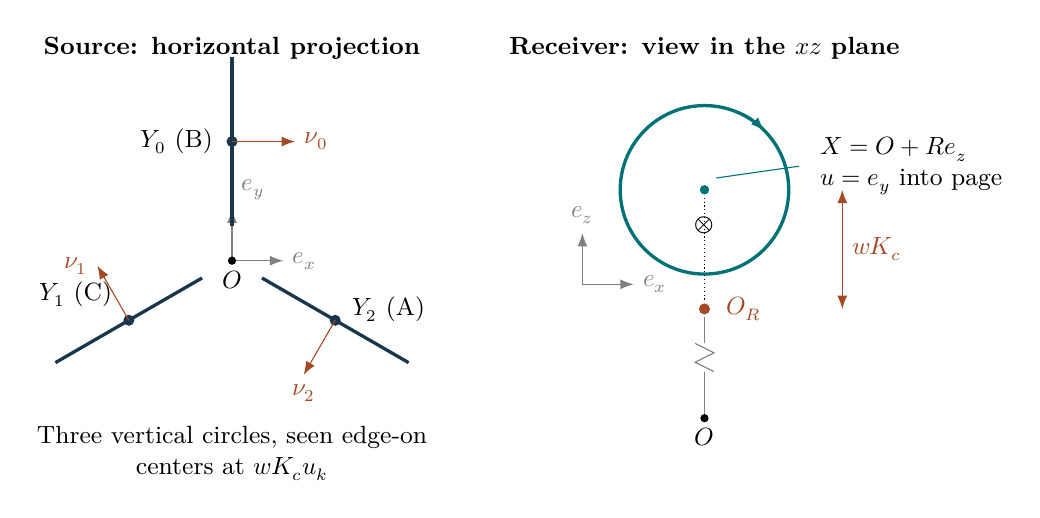
\begin{tikzpicture}[x=1cm,y=1cm,>=Latex,font=\small]
\node[font=\small\bfseries] at(0,2.7) {Source: horizontal projection};
\draw[->,gray] (0,0)--(.65,0) node[right] {$e_x$};
\draw[->,gray] (0,0)--(0,.65) node[above right] {$e_y$};
\fill (0,0) circle(1.5pt);\node[below] at(0,0) {$O$};
\draw[ink,very thick] (0,.44)--(0,2.59);
\draw[ink,very thick] (.381,-.22)--(2.243,-1.295);
\draw[ink,very thick] (-.381,-.22)--(-2.243,-1.295);
\fill[ink] (0,1.513) circle(2pt);
\fill[ink] (1.310,-.757) circle(2pt);
\fill[ink] (-1.310,-.757) circle(2pt);
\node[anchor=east] at(-.12,1.513) {$Y_0$ (B)};
\node[anchor=west] at(1.4,-.62) {$Y_2$ (A)};
\node[anchor=east] at(-1.4,-.43) {$Y_1$ (C)};
\draw[->,rust] (0,1.513)--(.8,1.513) node[right] {$\nu_0$};
\draw[->,rust] (1.310,-.757)--(.91,-1.45) node[below] {$\nu_2$};
\draw[->,rust] (-1.310,-.757)--(-1.71,-.064) node[left] {$\nu_1$};
\node[align=center] at(0,-2.45) {Three vertical circles, seen edge-on\\centers at $wK_cu_k$};
\node[font=\small\bfseries] at(6,2.7) {Receiver: view in the $xz$ plane};
\draw[teal,very thick] (6,.9) circle(1.07);
\draw[->,teal] (6,1.97) arc[start angle=90,end angle=45,radius=1.07];
\fill[teal] (6,.9) circle(1.7pt);
\node[anchor=west,align=left] at(7.35,1.2) {$X=O+Re_z$\\$u=e_y$ into page};
\draw[teal] (6.15,1.05)--(7.2,1.2);
\node at(6,.45) {$\otimes$};
\draw[densely dotted] (6,.8)--(6,-.5);
\fill[rust] (6,-.613) circle(2pt);
\node[anchor=west,rust] at(6.15,-.613) {$O_R$};
\draw[<->,rust] (7.75,.9)--node[right] {$wK_c$}(7.75,-.613);
\draw[gray] (6,-.72)--(6,-1.05);
\draw[gray] (5.88,-1.05)--(6.12,-1.17)--(5.88,-1.29)--(6.12,-1.41);
\draw[gray] (6,-1.42)--(6,-2);
\fill (6,-2) circle(1.5pt);\node[below] at(6,-2) {$O$};
\draw[->,gray] (4.45,-.3)--(5.1,-.3) node[right] {$e_x$};
\draw[->,gray] (4.45,-.3)--(4.45,.35) node[above] {$e_z$};
\end{tikzpicture}
}
\caption{Geometry of the native-launch test. Left: the three source circles have distinct centers; their horizontal projections are radial segments because their planes are vertical. The arrows are the fixed oriented normals, not signs of the launched means. Right: the actual receiving circle lies in the xz plane with increasing theta clockwise in this view, normal \(+\ey\), and \(b=wR_\Gamma\). The long R separation is broken schematically; the picture is not to scale. The body center is displaced by \(wK_c\) from the circle center.}\label{fig:native}
\end{figure}

Let \(\ell_0=wK_c\) and \(J_*=\sum_i|j_i|\). If \(R>\ell_0+a+b\), the whole receiving disk is separated from every filled source disk by at least
\begin{equation}\label{eq:clearance}
\delta_D\ge R-\ell_0-a-b>0.
\end{equation}
The full copies and their circles are also separated by enclosing balls in the range \(R\ge100w\). All three distinct source centers remain in the exact C6 integrals.

Their aggregate leading moment about O is \(\pi a^2\alpha W_0\). At \(X=O+R\ez\), the leading curl field has y-component
\begin{equation}\label{eq:leadingcomponent}
h_{\rm lead}=-\frac{g_oa^2\alpha W_{0y}}{4R^3},\qquad
W_{0y}=\frac{57}{400000}>0.
\end{equation}
The centered \(O(r^{-5})\) error of one loop cannot be reused unchanged about O: translations of the three source centers can give an \(O(R^{-4})\) correction.

\begin{theorem}[A signed finite-radius native readout]\label{thm:native}
For \(\alpha\ne0\), placement \eqref{eq:receiverplacement}--\eqref{eq:nativecontour}, and every \(R\ge100w\),
\begin{equation}\label{eq:thirdbound}
|S_b-h_{\rm lead}|<\tfrac13|h_{\rm lead}|.
\end{equation}
For positive alpha the launch reading is negative; its conjugate is exactly the opposite and positive. The radius remains \(b=wR_\Gamma\).
\end{theorem}
\begin{proof}
The estimate has three contributions:
\begin{align}
|S_b-h_{\rm lead}|&\le\mathcal E(R),\label{eq:Ebound}\\
\mathcal E(R)&=g_oJ_*\left[
\frac{6a^2\ell_0}{(R-\ell_0)^4}
+\frac{3a^4}{2(R-\ell_0-a)^5}
+\frac{3a^2b^2}{2(R-\ell_0-a-b)^5}
\right].\notag
\end{align}
For the translation term, direct differentiation of \eqref{eq:kernelG} gives
\begin{equation}\label{eq:DG}
D_vG(x)=|x|^{-4}
\{-15(n\cdot v)nn^T+3(n\cdot v)I+3(nv^T+vn^T)\},
\end{equation}
so \(\norm{D_vG(x)}_{\rm op}\le24|v|/|x|^4\). The segment from \(X-O\) to \(X-Y_i\) stays outside radius \(R-\ell_0\); multiply by \(g_o|j_i|a^2/4\) and sum. The centered remainder \eqref{eq:remainder} gives the second term. Disk averaging \eqref{eq:diskaveragebound}, with \eqref{eq:clearance}, gives the third. Equation~\eqref{eq:Ebound} bounds the \emph{area-averaged} reading relative to the central leading component; it is not a pointwise error bound replacing all disk points by the center.

From the exact launched weights,
\begin{equation}\label{eq:Jratio}
\frac{J_*}{|\alpha|W_{0y}}=\frac{57002\sqrt3}{85500}<\frac65,\qquad
0<K_c<1,\quad \tfrac12<R_\Gamma<1.
\end{equation}
Put \(q=w/R\le1/100\). Dividing \eqref{eq:Ebound} by \(|h_{\rm lead}|\) yields
\begin{equation}\label{eq:rationalbound}
\frac{\mathcal E(R)}{|h_{\rm lead}|}<
\frac{144q}{5(1-q)^4}
+\frac{36q^2}{5}\{(1-2q)^{-5}+(1-3q)^{-5}\}.
\end{equation}
Each term increases on this interval. At \(q=1/100\) the right side is
\begin{equation}\label{eq:rationalvalue}
\frac{7804605427237675733225000}{25890315358991719010197977}
=0.301448835945798\ldots<\frac13.
\end{equation}
This proves \eqref{eq:thirdbound}. The exact integral is linear in all three means; conjugation reverses them all and hence reverses the full finite-radius reading.
\end{proof}
The range is sufficient and configuration-specific, not an optimal threshold. This native placement does not generally have zero V at X; the zero-center result belongs to the separate coaxial control.

\begin{table}[tbp]\centering\small
\begin{tabular}{@{}rrrr@{}}\toprule
\(R/w\)&Finite contour \(S_b\)&\(h_{\rm lead}\)&\(\mathcal E(R)\)\\\midrule
100&\(-1.0251976124210\,10^{-11}\)&\(-1.0252192872890\,10^{-11}\)&\(2.2207690784546\,10^{-12}\)\\
200&\(-1.2815173359258\,10^{-12}\)&\(-1.2815241091113\,10^{-12}\)&\(1.3656205101897\,10^{-13}\)\\\bottomrule
\end{tabular}
\caption{Saved numerical corroboration at \(g_o=\alpha=w=1\), using all three source circles. Angular resolutions 64, 128 and 256 and a disk integration of H agree in the GM06 evidence. The all-distance guarantee is the analytic bound \eqref{eq:rationalbound}--\eqref{eq:rationalvalue}.}\label{tab:native}
\end{table}

\subsection{The 1,024-sample statement has its own premises}
Suppose N additional equally spaced points on the receiving rim have exact signed vector records \(v_k=B_k^TV(q(\theta_k))\). Reassemble the vectors before combining frames:
\begin{equation}\label{eq:SN}
S_{b,N}=\frac{2}{bN}\sum_{k=0}^{N-1}t(\theta_k)\cdot B_kv_k,\qquad
\theta_k=2\pi k/N.
\end{equation}
If \(F(\theta)=V(q(\theta))\cdot t(\theta)\) is \(C^2\), the composite trapezoidal error is
\begin{equation}\label{eq:quadratureerror}
|S_{b,N}-S_b|\le\frac{2\pi^2}{3bN^2}\sup|F''|.
\end{equation}
Using \(q'=bt,q''=-b(e_1\cos\theta+e_2\sin\theta)\), and the kernel derivatives,
\begin{equation}\label{eq:Fsecond}
\sup|F''|\le\frac{g_oaJ_*}{2}
\left(\frac{2b^2}{\delta^3}+\frac{3b}{\delta^2}+\frac1\delta\right)
\end{equation}
for contour-wire clearance delta. Indeed \(|F''|\le b^2M_{2,V}+3bM_{1,V}+M_{0,V}\), while inverse-distance derivatives are bounded by \(2/\delta^3,1/\delta^2,1/\delta\).

At \(R=100w\), use \(\delta>97w\), \(a=b>w/2\), \(a=b<w\), \eqref{eq:Jratio} and \(\pi^2<10\). For N=1024,
\begin{equation}\label{eq:1024}
\frac{|S_{b,1024}-S_b|}{|h_{\rm lead}|}
<
\frac{64000000}{1024^2}
\left(\frac2{97^3}+\frac3{97^2}+\frac1{97}\right)<\frac23.
\end{equation}
The continuous reading has magnitude greater than \(2|h_{\rm lead}|/3\), so the discrete sum retains its sign. These are new contour samples, not the old array's body-center sites. The result is for \(R=100w\), not fixed N at every larger R. Tangent measurement error at most epsilon per sample adds at most \(2\epsilon/b\); no instrument precision is presumed. The one-sample coaxial corollary has a separate symmetry premise.

\subsection{Arrival and completion of the steady reading}\label{sec:delay}
For a source history that vanishes before \(t_0\) and is constant after the jump, define on the rim C
\begin{equation}\label{eq:delays}
\tau_{\min}^{C}=\min_{P\in C,i,s}\frac{|P-\gamma_i(s)|}{c_e},
\qquad
\tau_{\max}^{C}=\max_{P\in C,i,s}\frac{|P-\gamma_i(s)|}{c_e}.
\end{equation}
The contour is silent before \(t_0+\tau_{\min}^C\). Its whole static record is available after the strict time \(t>t_0+\tau_{\max}^C\), provided the sources remain constant. Intermediate records need their actual delayed histories; the earliest permitted contribution does not guarantee a nonzero aggregate at the first-arrival instant.

The reviewed timing correction is
\begin{equation}\label{eq:delaymaxequal}
\boxed{\tau_{\max}^{D_b}=\tau_{\max}^{C}.}
\end{equation}
For a fixed source point, every interior disk point is a convex combination of two rim points on a chord. Convexity of distance bounds its distance by the larger endpoint distance. Maximizing over source points proves equality. Disk and rim minima can differ. The strict post-maximum inequality gives a neighborhood where all delayed arguments lie in the smooth plateau, justifying Stokes and differentiation over the disk.

For coaxial circles the common latest delay is
\(\sqrt{z^2+(a+b)^2}/c_e\), while the rim and disk minima are respectively
\(\sqrt{z^2+(a-b)^2}/c_e\) and \(\sqrt{z^2+(a-b)_+^2}/c_e\).
For the native placement, sufficient bounds are
\begin{equation}\label{eq:delaybounds}
\tau_{\min}^{D_b}\ge\frac{R-\ell_0-a-b}{c_e},\qquad
\tau_{\max}^{D_b}=\tau_{\max}^{C}\le\frac{R+\ell_0+a+b}{c_e}.
\end{equation}
At \(R=100w\) the ceiling is \(101.82961419736\,w/c_e\). This is the adopted straight-delay clock, not a derived electromagnetic speed or native physical duration.

\section{What reaches the receiver, and what remains open}\label{sec:scope}
\subsection{A scalar component, not a full vector}
The exact new observable is the disk average \eqref{eq:stokes}; \eqref{eq:areaerror} controls its difference from the center component. In the native test it is a signed y-component average. This already distinguishes the two launched preparations.

Even hypothetical three-normal measurements at a common point would have only rank two:
\begin{equation}\label{eq:ranktwo}
\sum_{k=0}^2\nu_k\nu_k^T=\frac32(I-\ez\ez^T).
\end{equation}
This is the body-local frame. For a copy rotated by Q, the ambient projector is
\(Q(I-\ez\ez^T)Q^T\). In local coordinates the inverse recovers
\(H_\perp=(2/3)\sum_k\nu_k(\nu_k\cdot H)\), not the third component.
The actual receiving circles also have different centers \(O_R+wK_cQ u_k\); their finite-area averages are not components of one common pointwise vector. A common-point or uniform-field reconstruction needs a further experiment or controlled gradient approximation. None is used here.

\subsection{Existing probes and the two WT paths}
Published complete-copy probes are center-sampled, with frames
\(B_k=[e_r(\phi_k),\ez,-e_\phi(\phi_k)]\)~\cite{PAIR,PAIRII}. The H and R fixtures have 84 distinct sites after accounting for their shared twelve-site ring. Their local triples must be reassembled by B before comparing spatial directions. They are not the added receiving-rim samples in \eqref{eq:SN}.

WT's six labeled broken arcs are specified by actual endpoints~\cite[setting, \texttt{eq:actualG}]{WT}:
\begin{equation}\label{eq:arcs}
G_k^+=[U_k,T_{2k+1}]\cup[T_{2k+1},U_{k+1}],\qquad
G_k^-=[L_k,B_{2k+1}]\cup[B_{2k+1},L_{k+1}].
\end{equation}
With cyclic endpoints, the upper arcs concatenate as
\(U_0,T_1,U_1,T_3,U_2,T_5,U_0\), and the lower as
\(L_0,B_1,L_1,B_3,L_2,B_5,L_0\). Thus they are two geometric six-edge closed paths, not one route inferred from the count six. Each is different from the tested receiving circle. The upper U vertices lie at height \(1/2\), while the T elbows lie at \(h_g=(\sqrt2-1)/2\); they do not lie in one plane.

The WT observation is a scalar-plus-vector field on the labeled arclength space \(G\). Its loaded receiving state obeys
\begin{equation}\label{eq:WTreceiver}
\beta_G\dot\zeta=\sqrt2 C_{\rm sp}c_{\rm in}
-C_{\rm sp}C_{\rm sp}^*\zeta,\qquad
(C_{\rm sp}v)(X)=\frac{g_o\sqrt M}{4\pi}
\int\frac{(v_p,\widehat t\,v_r)(s,X)}{d_X(s)}\dd s .
\end{equation}
This mixes source labels at each X; it does not form an oriented receiving-path integral. Such an integral could be added as a bounded functional of a continuous arc record, with a chosen traversal. A flux interpretation would also require a clear spanning surface. The existing loaded \(\zeta\) is not generally the passive C6 output and is not a second native complex triad.

\subsection{The completed correspondence}
Table~\ref{tab:status} separates definitions, adopted comparison laws, proposed additions and deductions. The model's fixed planes and chirality supply a precise geometric direction. They do not by themselves provide a source, a magnetic instrument or a force on another native state.

\begin{table}[tbp]\centering\small
\begin{tabularx}{\textwidth}{@{}>{\raggedright\arraybackslash}p{.22\textwidth}Y@{}}\toprule
Status&Content and boundary\\\midrule
Native and geometric&
The unchanged F, \(C=\Re\Omega\times\Im\Omega\), \(W=TC\), three allowed circle normals and their distinct centers.\\[3pt]
Adopted comparison&
C1 carrier, C6 delayed vector observation and the already declared RX/WT extensions. C6 alone is passive.\\[3pt]
Proposed here&
Three simultaneous carriers with the mean impulse \eqref{eq:jump}; signed tangent sampling and contour aggregation \eqref{eq:sensor}.\\[3pt]
Established conditionally&
Coaxial sign and its one-sample corollary; minimum means and exact launch work; finite-area native sign for \(R\ge100w\); the specified finite-sample and delay certificates.\\[3pt]
Unprovided&
An internal source donor, physical calibration and clock, an input law changing a second native triad, and reciprocal receiving work or force.\\\bottomrule
\end{tabularx}
\caption{Scope of the combined GM04--GM06 correspondence. The successful sensor is passive, and the benchmark source remains externally worked.}\label{tab:status}
\end{table}

The two tests answer distinct parts of the source-to-readout question. The coaxial control proves that a zero center vector can coexist with a nonzero signed loop measurement. The native control proves that the specified source impulse can place the native planar moment into a resolvable signed finite-radius observation. Its cost is \eqref{eq:launchcost}, and its readout is the scalar \eqref{eq:stokes}. An autonomous response of a second triad is a subsequent constitutive choice, not an unperformed step in either proof.

\paragraph{Research provenance.}
Hilmir Frímann Halldórsson is the author. GPT supplied analytical proposals and project-internal review; Codex supplied source verification, mathematical checking and manuscript preparation. These tools are not coauthors. The accepted investigations and their corrections are preserved unchanged, with exact primary-source identities and a manuscript crosswalk. This publication introduces no new scientific run, native coefficient or production change. Existing source-specific notices remain in force; no new blanket reuse licence is granted.

\appendix
\section{The differentiated-kernel certificate}\label{app:kernel}
For completeness, the estimate used in \eqref{eq:remainder} and \eqref{eq:diskaveragebound} can be proved directly~\cite[section 3]{GM04}:
\begin{equation}\label{eq:D2G}
\norm{D_v^2\Hess(|x|^{-1})}_{\rm op}\le\frac{24|v|^2}{|x|^5},
\qquad x\ne0.
\end{equation}
By rotation and homogeneity, put \(x/|x|=E_3\) and a unit v in the \(E_1,E_3\) plane. Write \(q=(v\cdot E_3)^2\in[0,1]\). After multiplication by \(|x|^5\), the matrix has the independent eigenvalue \(3-15q\in[-12,3]\) and the block
\begin{equation}\label{eq:block}
M(q)=
\begin{pmatrix}
9-21q&-24\sqrt{q(1-q)}\\
-24\sqrt{q(1-q)}&36q-12
\end{pmatrix}.
\end{equation}
The sign of the off-diagonal term can change with the sign of the components of v, without changing the following determinants.

The diagonal entries of \(24I-M\) are \(15+21q\) and \(36(1-q)\); its determinant is \(180(1-q)(3+q)\). The diagonal entries of \(24I+M\) are \(33-21q\ge12\) and \(12+36q\ge12\); its determinant is \(396+180q(2-q)\ge396\). Both matrices are positive semidefinite. Hence all eigenvalues of M lie between -24 and 24, proving \eqref{eq:D2G}. Taylor's integral remainder contributes one half, and integration of \(|\rho|^2\) over the radius-a disk gives \(\pi a^4/2\). Multiplication by \(g_o|j|/(4\pi)\) yields the coefficient \(3g_o|j|a^4/2\) in \eqref{eq:remainder}.

\section{Evidence and claim correspondence}\label{app:evidence}
The public edition preserves the accepted GM04--GM06 scientific derivations, reviews, check programs, saved results and exact primary sources. Complete original submission archives remain in the local record. Flat copies of 24 primary sources retain their SHA-256 and Git blob identities. The contextual GM01--GM03 manuscript is the author-approved edition~\cite{GM123}; its commit and PDF identity are retained in the preserved receipt.

\begin{table}[htbp]\centering\small
\begin{tabularx}{\textwidth}{@{}p{.41\textwidth}Y@{}}\toprule
Manuscript claim&Accepted evidence location\\\midrule
\eqref{eq:curl}--\eqref{eq:remainder}; Appendix~\ref{app:kernel}&
GM04 (6)--(15), exact curl, dipole tensor and uniform derivative bound.\\[3pt]
\eqref{eq:C1}--\eqref{eq:WTmean}&
GM04 (16)--(26), invariant, Fourier witness, old-port null pair and WT returning-wave qualification.\\[3pt]
\eqref{eq:lift}--\eqref{eq:launchcost}&
Reviewed GM05 (7)--(17), (22)--(26), minimum lift, errors, exact native launch and signed work.\\[3pt]
\eqref{eq:offsetreversal}--\eqref{eq:offsetwork}&
GM05 corrected section 4 and six review controls; persistent preloaded common offset.\\[3pt]
Theorem~\ref{thm:coaxial}; Corollary~\ref{cor:onesample}&
Reviewed GM06 (15)--(19); the GM06 review's rotational-symmetry corollary.\\[3pt]
Theorem~\ref{thm:native}; \eqref{eq:1024}&
Reviewed GM06 (20)--(31), exact placement, area-average certificate and finite-sampling bound.\\[3pt]
\eqref{eq:delaymaxequal}; \eqref{eq:ranktwo}&
Reviewed GM06 section 6 and section 5: equal latest delays and body-local projector clarification.\\[3pt]
Tables~\ref{tab:coax}--\ref{tab:native}&
GM06 saved check record; numerical corroboration only, with source and disk quadratures.\\\bottomrule
\end{tabularx}
\caption{Compact claim correspondence. The external crosswalk resolves these entries to manuscript labels, pages, exact files and primary equations.}\label{tab:crosswalk}
\end{table}

The prior scientific checks remain saved evidence, rather than new manuscript computations. GM04 has 78 heterogeneous checks, submitted GM05 has 62 with six additional review controls, and GM06 has 59 groups including its grouped review-control and byte checks. These counts are not theorem counts. The written proofs supply the continuum statements. Manuscript verification concerns transcription, source preservation, equation/citation resolution, embedded fonts, successful Windows compilation and visual inspection of every final page.

\begin{thebibliography}{10}
\bibitem{GM04}
H.~F.~Halldórsson, with GPT and Codex research assistance.
\emph{Native magnetic field transfer assessment}.
GM04 accepted local investigation, 20 November 2026.
Preserved derivation: \texttt{GM04\_DERIVATIONS.md}; exact evidence path in the accompanying source crosswalk.

\bibitem{GM05}
H.~F.~Halldórsson, with GPT and Codex research assistance.
\emph{Native moment to loop circulation}.
GM05 accepted with the section 4 common-offset correction, 20 November 2026.
Preserved authority: \texttt{GM05\_DERIVATIONS\_REVIEWED.md} and its acceptance note.

\bibitem{GM06}
H.~F.~Halldórsson, with GPT and Codex research assistance.
\emph{Passive signed loop reception}.
GM06 accepted with the latest-delay and frame clarifications, 20 November 2026.
Preserved authority: \texttt{GM06\_DERIVATIONS\_REVIEWED.md} and its acceptance note.

\bibitem{GM123}
H.~F.~Halldórsson.
\emph{Gravitational and magnetic source correspondence in the Tri-Octagon model: energy exchange and a switch-off test}.
Research edition v0.1 (2026).
\href{https://github.com/pzychozen/trioctagon-physics/blob/01841cac667cc0967de932aaeec0e74632f80e40/papers/GRAVITY_MAGNETISM_SOURCE_CORRESPONDENCE/publication/v0.1/output/GM01_GM03_COMBINED_PAPER_v0.1.pdf}{Author-approved contextual paper}, GM01--GM03.

\bibitem{G}
H.~F.~Halldórsson.
\emph{Geometry-Attached Axial Observables, Period-Doubling, and Certified Entrance Capture in the Tri-Octagon Map}.
Paper G, v0.1.1 (2026).
\href{https://github.com/pzychozen/trioctagon-physics/blob/ca22652dc000ca2b16419c1af4167918eab1ae94/papers/PAPER_G/v0.1.1/source/paper_g.tex}{Pinned source}; labels \texttt{eq:SA}, \texttt{eq:T}, \texttt{eq:W}.

\bibitem{PAIR}
H.~F.~Halldórsson.
\emph{Paired-Gap Geometry and Toroidal Observation Maps}.
Research edition v0.1.1 (2026).
\href{https://github.com/pzychozen/trioctagon-physics/blob/ca22652dc000ca2b16419c1af4167918eab1ae94/SRG_REDISCOVERY/PAPERS/PAIRED_GAP_GEOMETRY_OBSERVATION/publication/v0.1.1/geometry.tex}{Pinned geometry}; labels \texttt{eq:circle}, \texttt{eq:frames}, \texttt{eq:placement}.

\bibitem{PAIRII}
H.~F.~Halldórsson.
\emph{Paired Driving and Exterior Identifiability}.
Research edition v0.1 (2026).
\href{https://github.com/pzychozen/trioctagon-physics/blob/ca22652dc000ca2b16419c1af4167918eab1ae94/SRG_REDISCOVERY/PAPERS/PAIRED_DRIVING_EXTERIOR_IDENTIFIABILITY/publication/v0.1/exterior.tex}{Pinned exterior observation}; \texttt{eq:C6}, \texttt{thm:history}.

\bibitem{INT}
H.~F.~Halldórsson.
\emph{Native Intensity Accounting and Conditional Carrier Crossings}.
Research edition v0.1 (2026).
\href{https://github.com/pzychozen/trioctagon-physics/blob/ca22652dc000ca2b16419c1af4167918eab1ae94/papers/NATIVE_INTENSITY_AND_CONDITIONAL_CARRIER_CROSSINGS/publication/v0.1/manuscript/carrier.tex}{Pinned carrier}; labels \texttt{eq:C1}, \texttt{eq:storage}, \texttt{eq:C6}.

\bibitem{RX}
H.~F.~Halldórsson.
\emph{A Reciprocal Chiral Exchange Extension of the Tri-Octagon Model}.
Research edition v0.1 (2026).
\href{https://github.com/pzychozen/trioctagon-physics/blob/ca22652dc000ca2b16419c1af4167918eab1ae94/papers/RECIPROCAL_CHIRAL_EXCHANGE/publication/v0.1/manuscript/candidate.tex}{Pinned candidate};
\href{https://github.com/pzychozen/trioctagon-physics/blob/ca22652dc000ca2b16419c1af4167918eab1ae94/papers/RECIPROCAL_CHIRAL_EXCHANGE/publication/v0.1/manuscript/hybrid.tex}{native map and hybrid account}.

\bibitem{WT}
H.~F.~Halldórsson.
\emph{Spatial Observation and Causal Transport with Storage in the Reciprocal Chiral Exchange Candidate}.
Research edition v0.1 (2026).
\href{https://github.com/pzychozen/trioctagon-physics/blob/ca22652dc000ca2b16419c1af4167918eab1ae94/papers/SPATIAL_WORK_CAUSAL_TRANSPORT/publication/v0.1/sections/02_setting.tex}{Pinned geometry and retained state};
\href{https://github.com/pzychozen/trioctagon-physics/blob/ca22652dc000ca2b16419c1af4167918eab1ae94/papers/SPATIAL_WORK_CAUSAL_TRANSPORT/publication/v0.1/sections/05_transport.tex}{transport and receiving equations}.
\end{thebibliography}

\end{document}
